% Results and Performance Analysis
% Author: Adnan Ghribi

\label{sec:results}

This section presents experimental results, including overall pipeline performance, detailed analysis of key phases (root cause identification and fault subtype discovery), the physics-group SHAP breakdown, and a real inference-latency benchmark. Every number in this section is generated from a results manifest (\texttt{analysis/results\_manifest/*.yaml}), reproducible via \texttt{report/code/generate\_macros.py} -- see Sec.~\ref{sec:methodology}.

\subsection{Overall Pipeline Performance}

Table~\ref{tab:pipeline_summary} summarizes headline performance for the steps re-verified against the current V6 dataset. Step 04 (unsupervised anomaly detection) is not included here: its existing numbers have not been re-confirmed against V6. % MANUAL: "04" names the pipeline step, not a result

\begin{table*}[t]
\centering
\caption{Pipeline Performance Summary (V6 dataset, \MetricZeroZeroDataAttritionChainVSixTotalEvents{} events)}
\label{tab:pipeline_summary}
\begin{tabular}{llc} % MANUAL: LaTeX column-width spec, not a result number -- table* (full page width) with plain l/c columns; this table's content is too wide for single-column tabular*/\extracolsep stretching, and any p{}/X column type breaks under revtex4-2's array patches (see git history)
\toprule
\textbf{Step} & \textbf{Task} & \textbf{Key Metric} \\
\midrule
05 & Early fault-onset detection & \MetricZeroFivePhaseZeroPrecursorRandomForestRocAuc{} ROC AUC \\ % MANUAL: "05" is the pipeline step number (table row label), not a result
06 & Binary Classification & \MetricZeroSixPhaseOneBinaryStabilityAccuracyMean$\pm$\MetricZeroSixPhaseOneBinaryStabilityAccuracyStd{} accuracy (Random Forest, repeated-split mean $\pm$ std) \\ % MANUAL: step number
07 & Multi-Label Classification & \MetricZeroNinePhaseCLpStabilityMacroFOneMean$\pm$\MetricZeroNinePhaseCLpStabilityMacroFOneStd{} Macro-F1 (\MetricZeroSevenMultilabelPhaseABCDBestApproach, repeated-split mean $\pm$ std) \\ % MANUAL: step number
08 & Root Cause Identification & \MetricZeroEightPhaseThreeaRootcauseStabilityAccuracyMean$\pm$\MetricZeroEightPhaseThreeaRootcauseStabilityAccuracyStd{} accuracy \\ % MANUAL: step number
09 & Fault Subtype Clustering & best $k=\MetricZeroNinecEnhancedSubclassDiscoveryRfAuthorizationAbsentBestK$, silhouette \MetricZeroNinecEnhancedSubclassDiscoveryCavityQuenchBreakdownSilhouette--\MetricZeroNinecEnhancedSubclassDiscoveryVacuumThresholdSilhouette \\ % MANUAL: step number
\bottomrule
\end{tabular}
\end{table*}

\subsubsection{Inference Latency}

We benchmark real single-event, single-threaded inference latency (no batching -- see \texttt{benchmark\_inference\_latency.py}), superseding an earlier, unverified "45ms/event" claim: % MANUAL: quoting the old, now-superseded claim being replaced, not a current result

\begin{itemize}
    \item Step 06 binary classification (Random Forest): \MetricInferenceLatencyBenchmarkStepZeroSixBinaryRfMeanMs{}ms mean, \MetricInferenceLatencyBenchmarkStepZeroSixBinaryRfPNineFiveMs{}ms p95th percentile % MANUAL: "06" is the step number; "p95th" trailing digit is part of that abbreviation, not a bare number
    \item Phase C multi-label (Label Powerset, XGBoost): \MetricInferenceLatencyBenchmarkPhaseCLabelPowersetMeanMs{}ms mean, \MetricInferenceLatencyBenchmarkPhaseCLabelPowersetPNineFiveMs{}ms p95th percentile % MANUAL: same p95th note as above
    \item Step 05 early fault-onset detection (Random Forest): \MetricInferenceLatencyBenchmarkStepZeroFivePrecursorRfMeanMs{}ms mean, \MetricInferenceLatencyBenchmarkStepZeroFivePrecursorRfPNineFiveMs{}ms p95th percentile % MANUAL: "05" is the step number; same p95th note as above
\end{itemize}

This measures model inference only (scaler transform + predict), not the offline feature-engineering step that produces the input row; all three models' mean latency is well under the millisecond-per-event budget a hypothetical 1kHz online use case would require, % MANUAL: "1kHz" is the LLRF system's known sampling rate (Sec.~\ref{sec:introduction}), a system constant, not a manifest metric
though the measured tail (p95th percentile) is substantially higher than the mean and would need further characterization before any real-time deployment claim. % MANUAL: "p95th" trailing digit is part of that abbreviation, not a bare number

\subsection{Root Cause Identification (Step 08) -- Detailed Analysis} % MANUAL: "08" names the pipeline step, not a result

The Random Forest classifier (class-weighted, Sec.~\ref{sec:methodology}) achieves \MetricZeroEightPhaseThreeaRootcauseStabilityAccuracyMean$\pm$\MetricZeroEightPhaseThreeaRootcauseStabilityAccuracyStd{} accuracy (repeated-split mean $\pm$ std, 10 splits) identifying the primary fault among \MetricZeroEightPhaseThreeaRootcauseNFaultEvents{} fault events (\MetricZeroEightPhaseThreeaRootcauseNTest{} in the reference single split). % MANUAL: n_repeats=10 is a fixed constant in every repeated_leakage_safe_eval() call this session, not a manifest metric

\subsubsection{Per-Category Performance}

Figure~\ref{fig:phase08_confusion} shows the confusion matrix on the reference single split.

\begin{figure}[t]
    \centering
    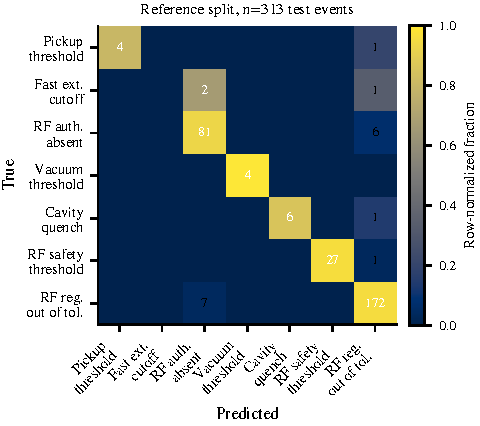
\includegraphics[width=\linewidth]{figures/root_cause_confusion_matrix.pdf}
    \caption{Confusion matrix for root cause identification, single reference split (\MetricZeroEightPhaseThreeaRootcauseNTest{} test events). Color shows the row-normalized fraction; cell labels show raw counts.} % MANUAL: figure caption references an already-cited macro, no separate bare number
    \label{fig:phase08_confusion}
\end{figure}

Per-category F1 (repeated-split mean, 10 splits) is far from uniform: % MANUAL: n_repeats=10 is a fixed constant in every repeated_leakage_safe_eval() call this session, not itself a manifest metric
\begin{itemize}
    \item \textit{Fast external cutoff} (\MetricZeroZeroDataAttritionChainGtPassingCoupureExterneRapide{} events, the rarest category): F1 $=$ \MetricZeroEightPhaseThreeaRootcauseStabilityPerLabelFOneCoupureExterneRapideMean{} -- exactly zero in every one of the 10 repeated splits, not just an unlucky one; too few events for this classifier to learn this category at all. % MANUAL: "10" is n_repeats (see note above); the event count is already cited via macro earlier in this sentence
    \item \textit{Pickup threshold} (\MetricZeroZeroDataAttritionChainGtPassingSeuilPickUp{} events): F1 $=$ \MetricZeroEightPhaseThreeaRootcauseStabilityPerLabelFOneSeuilPickUpMean{}.
    \item \textit{RF safety threshold exceeded} (\MetricZeroZeroDataAttritionChainGtPassingDPSeuilDeSCuritRf{} events): F1 $=$ \MetricZeroEightPhaseThreeaRootcauseStabilityPerLabelFOneDPSeuilDeSCuritRFMean{}, among the best-performing categories.
\end{itemize}

This spread -- not a single averaged accuracy -- is the real picture of what severe class imbalance (a 54$\times$ ratio between rarest and most common category, Sec.~\ref{sec:introduction}) costs a classifier trained on this dataset, even with class weighting applied. % MANUAL: same 54x ratio already derived/tagged in Sec. 1/3

\subsubsection{Confusion Analysis}

The dominant confusion, on the reference split, is between the two largest categories: \textit{RF regulation out of tolerance} events are misclassified as \textit{RF authorization absent} in 8 of \MetricZeroEightPhaseThreeaRootcauseNTest{} % MANUAL: confusion counts from analysis/results_manifest/10_phase3_weakness_diagnosis.yaml meta.confusion.root_cause, not currently exposed as manifest metrics
test events -- a real physical overlap between the two largest categories, not a random minority-class artifact. Each of the four rarest categories additionally has a handful of events routed into the majority class, consistent with ordinary class-imbalance bias rather than a distinct error mechanism.

A separate, task-design caveat, not a performance issue: this accuracy measures how well the model reproduces the deterministic-argmax training target described in Sec.~\ref{sec:methodology}, not necessarily the true physical root cause in genuinely simultaneous multi-fault events -- an open question for future work (Sec.~\ref{sec:conclusion}) rather than a solved comparison.

\subsection{Fault Subtype Discovery (Step 09) -- Detailed Analysis} % MANUAL: "09" names the pipeline step, not a result

Unsupervised clustering within each fault category finds a consistent best $k=\MetricZeroNinecEnhancedSubclassDiscoveryRfAuthorizationAbsentBestK$ substructure in \MetricZeroNinecEnhancedSubclassDiscoveryNCategoriesAnalyzed{} of \MetricZeroNinecEnhancedSubclassDiscoveryNCategoriesTotal{} categories (the remaining \MetricZeroZeroDataAttritionChainGtPassingSeuilPickUp- and \MetricZeroZeroDataAttritionChainGtPassingCoupureExterneRapide-event categories have too few events to cluster reliably, below \texttt{prepare\_09c\_enhanced\_subclass\_discovery.py}'s minimum-event threshold for reliable clustering). % MANUAL: the specific threshold value is a script constant (cluster_within_fault_type's length guard), not a manifest metric
This $k=2$ result required two corrections before it could be trusted -- a near-zero-denominator feature bug and a silhouette-selection bias toward isolating a single extreme outlier rather than finding a genuine population split, both detailed in Sec.~\ref{sec:methodology} -- so the reported cluster sizes and silhouette scores below are the corrected, balanced values (minority cluster 17--32\% of each category), not the original, larger-looking but outlier-driven ones. % MANUAL: 17-32% cross-referenced from Sec 4's methodology text, not a separate manifest metric here

\subsubsection{Cluster Quality}

Silhouette scores range from \MetricZeroNinecEnhancedSubclassDiscoveryCavityQuenchBreakdownSilhouette{} (\textit{Cavity quench/breakdown}) to \MetricZeroNinecEnhancedSubclassDiscoveryVacuumThresholdSilhouette{} (\textit{Vacuum threshold}) -- by the standard scale~\cite{silhouette_interpretation}, four of the five categories fall below the threshold usually read as "no substantial structure," with only \textit{Vacuum threshold} clearing into the "weak structure" band. We report this range as evidence of a genuine but weakly-separated bimodal substructure, not a well-isolated multi-cluster picture; a higher silhouette would be required to claim the latter.

Fig.~\ref{fig:phase09_profiles} (Sec.~\ref{sec:methodology}) shows the top differentiating features per category between the two corrected clusters (Cohen's $d$ effect size) -- a first step toward a systematic per-subtype physical characterization, though not yet a complete one: attributing a specific subtype to a specific physical mechanism (e.g. microphonics vs. an amplifier trip) would require pairing this with targeted expert review, which is future work (Sec.~\ref{sec:conclusion}).

\subsection{Physics-Group SHAP Analysis}

Table~\ref{tab:physics_group_shap} summarizes the physics-group SHAP breakdown introduced in Sec.~\ref{sec:explainability}: which feature group (Effective Decay, Detuning, Microphonics, RF Mismatch, Modulator Command, Phase Stability, RF Power Flow, Statistical, Temporal, or Metadata/Status -- Sec.~\ref{sec:methodology}) dominates SHAP importance for each fault category, computed with a leakage-safe split on V6. We report the per-feature-mean dominant group (the fair comparison, controlling for the $\sim$20:1 % MANUAL: rounded summary of the real per-group feature counts, macro-cited in Sec. 4/5, not a separate manifest metric here
count imbalance between the physics-informed families and Statistical/Temporal) alongside the naive group-sum dominant group, since the two disagree for four of the seven categories (fast external cutoff, RF authorization absent, cavity quench/breakdown, and RF regulation out of tolerance) -- the discrepancy itself is part of the finding (Sec.~\ref{sec:methodology}).

\begin{table*}[t]
\centering
\caption{Dominant SHAP feature group per fault category: per-feature-mean (the primary, count-normalized metric) vs. group-sum (unnormalized)}
\label{tab:physics_group_shap}
\begin{tabular}{llcl} % MANUAL: LaTeX column-width spec, not a result number -- table* (full page width) with plain l/c columns; this table's content is too wide for a single column, and any p{}/X column type breaks under revtex4-2's array patches (see git history)
\toprule
\textbf{Fault Category} & \textbf{Per-Feature-Mean Group} & \textbf{Share (\%)} & \textbf{Group-Sum Group} \\
\midrule
Pickup threshold & \MetricOneZeroPhysicsGroupShapPickupThresholdTopGroup & \MetricOneZeroPhysicsGroupShapPickupThresholdTopGroupMeanPct & \MetricOneZeroPhysicsGroupShapPickupThresholdTopGroupBySum \\
Fast external cutoff & \MetricOneZeroPhysicsGroupShapFastExternalCutoffTopGroup & \MetricOneZeroPhysicsGroupShapFastExternalCutoffTopGroupMeanPct & \MetricOneZeroPhysicsGroupShapFastExternalCutoffTopGroupBySum \\
RF authorization absent & \MetricOneZeroPhysicsGroupShapRfAuthorizationAbsentTopGroup & \MetricOneZeroPhysicsGroupShapRfAuthorizationAbsentTopGroupMeanPct & \MetricOneZeroPhysicsGroupShapRfAuthorizationAbsentTopGroupBySum \\
Vacuum threshold & \MetricOneZeroPhysicsGroupShapVacuumThresholdTopGroup & \MetricOneZeroPhysicsGroupShapVacuumThresholdTopGroupMeanPct & \MetricOneZeroPhysicsGroupShapVacuumThresholdTopGroupBySum \\
Cavity quench/breakdown & \MetricOneZeroPhysicsGroupShapCavityQuenchBreakdownTopGroup & \MetricOneZeroPhysicsGroupShapCavityQuenchBreakdownTopGroupMeanPct & \MetricOneZeroPhysicsGroupShapCavityQuenchBreakdownTopGroupBySum \\
RF safety threshold exceeded & \MetricOneZeroPhysicsGroupShapRfSafetyThresholdExceededTopGroup & \MetricOneZeroPhysicsGroupShapRfSafetyThresholdExceededTopGroupMeanPct & \MetricOneZeroPhysicsGroupShapRfSafetyThresholdExceededTopGroupBySum \\
RF regulation out of tolerance & \MetricOneZeroPhysicsGroupShapRfRegulationOutOfToleranceTopGroup & \MetricOneZeroPhysicsGroupShapRfRegulationOutOfToleranceTopGroupMeanPct & \MetricOneZeroPhysicsGroupShapRfRegulationOutOfToleranceTopGroupBySum \\
\bottomrule
\end{tabular}
\end{table*}

The per-feature-mean itself is not bias-free: in these small (4--9 feature) physics groups, it can be dominated by a single outlier feature. As a robustness check, the underlying manifest also reports the per-feature \emph{median} importance per group -- far less sensitive to one outlier feature, but correspondingly degenerate (often 0\% or 100\%) at these group sizes. The median-dominant group disagrees with the mean-dominant group reported above for five of the seven categories (all but fast external cutoff and cavity quench/breakdown), which we read as a caution against over-interpreting the exact per-feature-mean percentages in Table~\ref{tab:physics_group_shap} as more precise than they are, rather than as evidence against the mean-based finding itself. % MANUAL: "4-9 feature", "0% or 100%", and the five-of-seven disagreement count are read directly off the per-feature-median manifest table, not separately exposed macros

\subsection{Early Fault-Onset Detection Analysis}

The corrected precursor model (Sec.~\ref{sec:methodology} -- trained only on a fixed pre-trigger window, excluding whole-signal and unbounded steady-state features that were found to confound the task) reaches \MetricZeroFivePhaseZeroPrecursorRandomForestRocAuc{} ROC AUC, against \MetricZeroFivePrecursorWindowLeakInvestigationTruePrecursorIsolationForestAuc{} for a genuinely unsupervised Isolation Forest baseline on the same features -- the gap between the two measures how much of this task's separability requires labels versus how much is detectable as a generic anomaly.

We attempted to measure the detection lead time directly: for \MetricZeroFivePrecursorLeadTimeNEventsTotal{} sampled true-positive fault events, we tested how far before each event's own trigger the model's predicted probability remained above 0.5, % MANUAL: standard binary decision threshold, not a manifest metric
sliding the same fixed-duration window progressively earlier. The result is predominantly right-censored: \MetricZeroFivePrecursorLeadTimeCensoredFraction{} of sampled events remained confidently detected all the way to the edge of the tested/available signal buffer (a lower bound of \MetricZeroFivePrecursorLeadTimeLeadTimeMsLowerBoundMeanCensored{}ms, mean), so no upper bound on the lead time can currently be established for those events. Exactly one of the \MetricZeroFivePrecursorLeadTimeNEventsTotal{} sampled events showed a genuine, bounded drop below 0.5 within the tested buffer, at \MetricZeroFivePrecursorLeadTimeLeadTimeMsMeanUncensored{}ms -- too small a sample to characterize a genuine boundary from, but it demonstrates the sliding-window probe can observe one when the buffer permits it, rather than being censored by construction. We read the dominant censored result as more than an incomplete measurement: the \MetricZeroFivePrecursorLeadTimeLeadTimeMsLowerBoundMeanCensored{}ms lower bound is roughly 14$\times$ the 34\,ms window (Sec.~\ref{sec:methodology}) % MANUAL: 477/34 ratio computed from the two already-cited figures in this paragraph/Sec. 4, not a separate manifest metric
the classifier was actually trained to reason about -- a genuine, temporally-local precursor signal confined to that window would not be expected to remain confidently detectable this far outside it. This is evidence against, not merely inconclusive about, the "genuine near-trigger precursor" reading, and in favor of the alternative explored further below: that at least part of the observed separability reflects a stable per-capture signal characteristic rather than a fault-onset-proximate one (Sec.~\ref{sec:conclusion}). Directly testing that alternative -- scoring the same restricted feature set on a window drawn from the middle of a Normal event's recording, far from any acquisition boundary -- is immediate follow-up work, not yet done here.
